%%%%%%%%%%%%%%%%%%%%%%%%%%%%%%%%%%%%%%%%%%%%%%%
%
% Template per Elaborato di Laurea
% DISI - Dipartimento di Ingegneria e Scienza dell’Informazione
%
% update 2015-09-10
%
% Per la generazione corretta del 
% pdflatex nome_file.tex
% bibtex nome_file.aux
% pdflatex nome_file.tex
% pdflatex nome_file.tex
%
%%%%%%%%%%%%%%%%%%%%%%%%%%%%%%%%%%%%%%%%%%%%%%%

% formato FRONTE RETRO
\documentclass[epsfig,a4paper,11pt,titlepage,twoside,openany]{book}
\usepackage{epsfig}
\usepackage{plain}
\usepackage{setspace}
\usepackage[paperheight=29.7cm,paperwidth=21cm,outer=1.5cm,inner=2.5cm,top=2cm,bottom=2cm]{geometry} % per definizione layout
\usepackage{titlesec} % per formato custom dei titoli dei capitoli

%%%%%%%%%%%%%%
% supporto lettere accentate
%
%\usepackage[latin1]{inputenc} % per Windows;
\usepackage[utf8x]{inputenc} % per Linux (richiede il pacchetto unicode);
%\usepackage[applemac]{inputenc} % per Mac.

\singlespacing

\usepackage[english]{babel}

% PACCHETTI AGGIUNTI, CHIEDI!!!!
\usepackage{url}
\usepackage[multiple]{footmisc}
\usepackage{amsmath}
\newcommand*\NewPage{\newpage\null\thispagestyle{empty}\newpage}

\usepackage[a-1b]{pdfx}

\begin{document}

  % nessuna numerazione
  \pagenumbering{gobble} 
  \pagestyle{plain}

\thispagestyle{empty}

\begin{center}
  \begin{figure}[h!]
    \centerline{
\psfig{file=marchio_unitrento_colore_it_202002.eps,width=0.6\textwidth}}
  \end{figure}

  \vspace{2 cm} 

  \LARGE{Department of Information Engineering and Computer Science\\}

  \vspace{1 cm} 
  \Large{Bachelor’s Degree in\\
    Computer Science
    %Informatica
    %Ingegneria dell'Informazione e delle Comunicazioni
    %Ingegneria dell'Informazione e Organizzazione d'Impresa
    %Ingegneria Elettronica e delle Telecomunicazioni
  }

  \vspace{2 cm} 
  \Large\textsc{Final dissertation\\} 
  \vspace{1 cm} 
  \Huge\textsc{Automatic generation of marketing personas from social media data\\}


  \vspace{2 cm} 
  \begin{tabular*}{\textwidth}{ c @{\extracolsep{\fill}} c }
  \Large{Supervisors} & \Large{Student}\\
  \Large{Alberto Montresor} & \Large{Nicola Farina}\\
  \Large{Carlo Caprini} & \\
  \end{tabular*}

  \vspace{2 cm} 

  \Large{Academic year 2020/2021}
  
\end{center}


  \clearpage
  \NewPage{}
 
%%%%%%%%%%%%%%%%%%%%%%%%%%%%%%%%%%%%%%%%%%%%%%%%%%%%%%%%%%%%%%%%%%%%%%%%%%
%%%%%%%%%%%%%%%%%%%%%%%%%%%%%%%%%%%%%%%%%%%%%%%%%%%%%%%%%%%%%%%%%%%%%%%%%%
%% Nota
%%%%%%%%%%%%%%%%%%%%%%%%%%%%%%%%%%%%%%%%%%%%%%%%%%%%%%%%%%%%%%%%%%%%%%%%%%
%% Sezione Ringraziamenti opzionale
%%%%%%%%%%%%%%%%%%%%%%%%%%%%%%%%%%%%%%%%%%%%%%%%%%%%%%%%%%%%%%%%%%%%%%%%%%
%%%%%%%%%%%%%%%%%%%%%%%%%%%%%%%%%%%%%%%%%%%%%%%%%%%%%%%%%%%%%%%%%%%%%%%%%%
  \thispagestyle{empty}

\begin{center}
  {\bf \Huge Acknowledgments}
\end{center}

\vspace{4cm}


\emph{I want to thank all the people that have supported me during these three years: my parents, who never failed to provide me with everything I needed and were always there for me; and my closest friends, who lightened my mood in my most stressful periods.}

\emph{A huge thank you goes also to the people that helped and guided me in writing this thesis: first of all, Daniele Miorandi and Carlo Caprini, who relentlessly offered me the best advice and support whenever I needed it during my internship; all the U-Hopper team, which unfortunately I could not meet in person due to Covid restrictions, but who still made me feel like I was working in such a friendly environment; and Alberto Montresor, who is responsible for introducing me to U-Hopper in the first place.}

  \clearpage
  \pagestyle{plain} % nessuna intestazione e pie pagina con numero al centro

  
  % inizio numerazione pagine in numeri arabi
  \mainmatter

%%%%%%%%%%%%%%%%%%%%%%%%%%%%%%%%%%%%%%%%%%%%%%%%%%%%%%%%%%%%%%%%%%%%%%%%%%
%%%%%%%%%%%%%%%%%%%%%%%%%%%%%%%%%%%%%%%%%%%%%%%%%%%%%%%%%%%%%%%%%%%%%%%%%%
%% Nota
%%%%%%%%%%%%%%%%%%%%%%%%%%%%%%%%%%%%%%%%%%%%%%%%%%%%%%%%%%%%%%%%%%%%%%%%%%
%% Si ricorda che il numero massimo di facciate e' 30.
%% Nel conteggio delle facciate sono incluse 
%%   indice
%%   sommario
%%   capitoli
%% Dal conteggio delle facciate sono escluse
%%   frontespizio
%%   ringraziamenti
%%   allegati    
%%%%%%%%%%%%%%%%%%%%%%%%%%%%%%%%%%%%%%%%%%%%%%%%%%%%%%%%%%%%%%%%%%%%%%%%%%
%%%%%%%%%%%%%%%%%%%%%%%%%%%%%%%%%%%%%%%%%%%%%%%%%%%%%%%%%%%%%%%%%%%%%%%%%%

    % indice
    \tableofcontents
    \clearpage
    
    
    % gruppo per definizone di successione capitoli senza interruzione di pagina
    \begingroup
      % nessuna interruzione di pagina tra capitoli
      % ridefinizione dei comandi di clear page
      \renewcommand{\cleardoublepage}{} 
      \renewcommand{\clearpage}{} 
      % redefinizione del formato del titolo del capitolo
      % da formato
      %   Capitolo X
      %   Titolo capitolo
      % a formato
      %   X   Titolo capitolo
      
      \titleformat{\chapter}
        {\normalfont\Huge\bfseries}{\thechapter}{1em}{}
        
      \titlespacing*{\chapter}{0pt}{0.59in}{0.02in}
      \titlespacing*{\section}{0pt}{0.20in}{0.02in}
      \titlespacing*{\subsection}{0pt}{0.10in}{0.02in}
      
      % abstract
      \chapter*{Abstract} % senza numerazione
\label{cha:abstract}
\addcontentsline{toc}{chapter}{Abstract} % da aggiungere comunque all'indice
Nowadays digital marketing heavily relies on the segmentation of an audience at both aggregated and at the single user's level. Personas are profiles of fictional users that "humanize data" by giving an identity to each audience segment; they are used by marketeers to better understand their customers and make marketing decisions for each customer segment in an efficient way. 

Personas are traditionally created manually, by collecting data through interviews and surveys and analyzing it in a lengthy and expensive process. For this reason, in the latest years, the concept of automatic persona generation has increased in popularity. Nonetheless, very few services exist that offer such a solution, and those that do exist share limitations in either how or what data is collected to create the personas.

The best and easiest place to look for data to build personas on is social media: they are one of the most used means of communication, and offer a great source of both demographics and behavioral data, which is precious in order to create meaningful personas. This work explores the possibility of using social media data as a source for creating marketing personas.

This thesis was developed at U-Hopper\footnote{\url{www.u-hopper.com}}, a company that specializes in big data analytics and artificial intelligence, and that is already present in the world of customer knowledge.

The proposed solution not only shows that automatic persona generation from social media data is feasible, but also that a system with high scalability, expandability and accuracy can be designed and implemented to fulfill that task. It uses several components, each with a specific task, from data collection, to data enrichment, all the way to clustering and persona generation. Many classifiers are employed to extract insights from the available data, which are then used to create customers segments. All the components are linked in a stream-processing architecture, which allows to avoid bottlenecks and achieve high separation of concerns. Finally, users are segmented with very good accuracy, precision and recall measures, all above 0.9.
      \NewPage{}
%%%%%%%%%%%%%%%%%%%%%%%%%%%%%%%%%%%%%%%%%%%%%%%%%%%%%%%%%%%%%%%%%%%%%%%%%%
%%%%%%%%%%%%%%%%%%%%%%%%%%%%%%%%%%%%%%%%%%%%%%%%%%%%%%%%%%%%%%%%%%%%%%%%%%
%% Nota
%%%%%%%%%%%%%%%%%%%%%%%%%%%%%%%%%%%%%%%%%%%%%%%%%%%%%%%%%%%%%%%%%%%%%%%%%%
%% Sommario e' un breve riassunto del lavoro svolto dove si descrive 
%% l’obiettivo, l’oggetto della tesi, le metodologie e 
%% le tecniche usate, i dati elaborati e la spiegazione delle conclusioni 
%% alle quali siete arrivati.
%% Il sommario dell’elaborato consiste al massimo di 3 pagine e deve contenere le seguenti informazioni: 
%%   contesto e motivazioni
%%   breve riassunto del problema affrontato
%%   tecniche utilizzate e/o sviluppate
%%   risultati raggiunti, sottolineando il contributo personale del laureando/a
%%%%%%%%%%%%%%%%%%%%%%%%%%%%%%%%%%%%%%%%%%%%%%%%%%%%%%%%%%%%%%%%%%%%%%%%%%
%%%%%%%%%%%%%%%%%%%%%%%%%%%%%%%%%%%%%%%%%%%%%%%%%%%%%%%%%%%%%%%%%%%%%%%%%%      
      
      %%%%%%%%%%%%%%%%%%%%%%%%%%%%%%%%
      % lista dei capitoli
      %
      % \input oppure \include
      %
      \chapter{Introduction}
\label{cha:intro}
This thesis has been developed at U-Hopper, during a 4-month period in which I was able to combine a work experience in a company with the writing of my bachelor's thesis. U-Hopper is a company that defines itself as a "Data Intelligence Lab", with an expertise on Big Data Analytics, Business Intelligence and Artificial Intelligence. Headquartered in Trento, it provides big data-enabled solutions and technologies, for which it received numerous awards throughout the years.

The company has brought its presence into the user profiling world by developing Tapoi\footnote{\url{www.tapoi.cloud}}, a service that makes heavy use of artificial intelligence and machine learning algorithms to provide human-centered insights on existing customers. The existence of Tapoi is what inspired the work of this thesis, which proposes to further humanize customer data in order to make marketing decisions that result in a better custom experience. What follows is a brief introduction of the problem at hand.

\section{Problem statement}
Marketing is a crucial aspect for the success of any brand offering a service. Especially in today's globalized market, good advertising and communication strategies are the key to stand out amongst the competitors. Ultimately, marketing boils down to one thing: knowing your customers. With this knowledge, a company can understand the actual needs of their clients and design solutions that will satisfy them, ultimately increasing profit. In fact, customers, now more than ever before, want a personalized experience when interacting with a brand, which spans throughout the whole interaction (from product recommendations, to tailored emails).

A popular way to achieve customer knowledge is through \textit{personas}. A persona is an imaginary person representing a real user segment, that is, a group of people that have similar characteristics. Their power is that they allow to abstract a high number of customers, even millions, into only a few, easy to read profiles. Marketing specialists and sales teams can then use the data contained in these personas to make informed decisions on their marketing campaigns and to design the aforementioned personalized experiences. 

Traditionally, these personas are built manually by marketing specialists based on the outcome of interviews, focus groups and surveys. This approach is lengthy and expensive, as it often involves direct contact with customers and manual processing of a lot of data. The purpose of this thesis is to explore the possibility of automating this process.

In particular, we propose the following research question: is it possible to automatically generate marketing personas for a brand or organization, based on public data available on the legal basis? Let us better define some terms:
\begin{itemize}
    \item \textbf{automatically}: the user is not required to make decisions nor possess knowledge on how to create personas in order to use the service;
    \item \textbf{publicly available data}: data that can be collected publicly. Some examples are: social media, like Twitter or Facebook; other websites, for example blogs or sector-specific services like GitHub; third party data, such as national surveys or company data;
    \item \textbf{legal base}: the service needs to be fully compliant with GPDR, the General Data Protection Regulation.
\end{itemize}

This thesis shows that fulfilling this task is indeed possible, and proposes a system design to carry it out, together with a working prototype for demonstration purposes.

\section{Personas}
\label{sec:personas}
Personas were first introduced by Alan Cooper in 1999 \cite{cooper2004inmates} in the context of software development. They are "\textit{fictitious, specific and concrete representations of target users}" \cite{pruitt2010persona} to be used throughout the design process. With time, the persona technique has expanded to other fields, such as design, marketing, healthcare \cite{vosbergen2015using}, and even games \cite{tychsen2008defining}.

Given the high number of use-cases for personas, the information they contain and the way data is collected cannot be uniquely specified and can vary significantly between each project. Regardless, some information is commonly found in most personas, as can be seen in many general-purpose persona templates found on the Internet. This includes: demographics, such as name, age, place of residence, marital status or living situation, profession, photo; and psychographics, like personality traits, hobbies, interests and opinions, values, lifestyle and habits, frustrations, needs and motivations.

\section{Outline}
This thesis is organized as follows: Chapter \ref{cha:art} presents the state of the art related to the persona creation process, which is needed to understand the current research problems and gaps. Chapter \ref{cha:design} describes the design solution, with particular focus on the logical components of the system and on data modeling. In Chapter \ref{cha:implementation}, the implementation choices are presented and justified, while in Chapter \ref{cha:evaluation} the implemented prototype is evaluated. Chapter \ref{cha:conclusions} concludes this thesis with some final remarks for future work.

      \newpage
      \chapter{State of the art}
\label{cha:art}
In this chapter, the state of the art regarding the creation of personas is presented. It is divided in four sections which reflect the main steps of the process:
\begin{enumerate}
    \item~\textbf{data collection}, which consists in getting data about the users on which personas are built;
    \item~\textbf{data enrichment}, which consists in analysing the previously collected data to extract additional insights.
    \item~\textbf{clustering}, which consists in identifying groups of similar users based on the characteristics obtained in the previous two steps;
    \item~\textbf{persona generation}, which consists in creating a persona for each identified group.
\end{enumerate}
Each section will cover the work that has been done so far, with emphasis on the latest developments in the use of enriched social media data. The current research problem of fully automating the whole process is tackled as well.

\section{Data collection}
\label{sec:collection}
In this section, the main data sources and methods used to create personas are presented in chronological order, starting from hands-on qualitative methods, followed by surveys and the latest developments with web data.

\subsection{Qualitative methods}
\label{subsec:qualitative}
Traditionally, data was collected using purely qualitative methods. Those can be split into two categories: implicit and explicit. Implicit methods are described by the concept "don't ask, observe" and include observations, field studies and, in part, usability tests~\cite{mulder2007approaches, pruitt2003personas, olsen2004persona}. Explicit methods rely instead on directly asking questions to users: the most used ones are interviews and focus groups~\cite{mulder2007approaches, pruitt2003personas, olsen2004persona}. All these interactions, whether implicit or explicit, have to be carefully crafted, usually by experts of the given research field, in order to gain useful insights to be later analysed. 

Because of their open-ended nature, qualitative methods allow researchers to explore user behaviour in depth, but they also come with some shortcomings:
\begin{itemize}
    \item~\textbf{small coverage}: the research is usually done with few users (10-20)~\cite{mulder2007approaches}. Thus, there is no evidence that personas actually represent the full user base~\cite{chapman2006personas};
    \item~\textbf{subjectivity}: interview results and related qualitative data are subjective by nature, and can also present biases from both users and researchers~\cite{mulder2007approaches}.
\end{itemize}

\subsection{Surveys}
\label{subsec:surveys}
With the aforementioned flaws in mind, the concept of data-driven personas was introduced. It consists in grounding personas in real, larger-scale data by using quantitative research methods alongside qualitative ones (or completely replacing the latter)~\cite{mulder2007approaches}. The most popular data sources to achieve this are surveys: 47\% of papers about data-driven personas development report their use~\cite{salminen2021survey}. They are easy to share, allow a broad exploration of the user base, and are easier to cluster than open-ended interview results.

R. Sinha was one among the first ones to report the use of surveys in 2003, when developing personas for a restaurant recommendation system~\cite{sinha2003persona}. She and her team crafted a survey after having identified 32 relevant dimensions of the restaurant experience, asking users to rate them on a five point Likert scale. The same approach was taken by McGinn and Kotamraju in 2008 \cite{mcginn2008data}, who spent three weeks designing a survey together with the stakeholders and got 1300 responses, much more data than qualitative methods can achieve. 

The use of surveys was further explored in an article by Tu et al. in 2010~\cite{tu2010combine}. They begin by proposing four steps for the persona creation process, with the first one reading: "\textit{gather user data (personal data, users' relationships with the product and users' goals and motivations) through large scale questionnaires and user survey}". They highlighted that the design of the questionnaire is crucial in order to get relevant dimensions for clustering, and that it should focus on capturing user behaviors, goals and motivations. To build theirs, they used a template designed by George Olsen in his article "\textit{Persona creation and usage toolkit}"~\cite{olsen2004persona}, but noted that it was difficult to fully adapt it to their situation, suggesting that a "universal" template may not exist.

\subsection{Web data}
\label{subsec:webdata}
The next development in data collection came with the popularization of web data. Almost 30\% of papers on data-driven personas report its use, and the number is increasing and surpassed that of surveys~\cite{salminen2021survey}. Web data includes sources such as social media platforms (e.g. YouTube~\cite{an2018imaginary}), online discussion forums~\cite{huh2016personas}, and online analytics (e.g. clickstream data~\cite{zhang2016data}). The increasing popularity of the web also resulted in larger datasets and survey samples, with an average size about five times that of the first surveys~\cite{salminen2021survey}.

An example of the use of online analytics was proposed by Zhang et al. in 2016~\cite{zhang2016data}. Clickstream data is defined as sequences of users' clicks (or taps) when using a product. Using it as a data source comes with the following benefits: clickstreams directly describe user behavior and workflow in a product; additionally, they are collected automatically without the need of human intervention; on top of that, the constant collection of clickstreams allows personas to be easily updated in case their workflows evolve over time. This approach is suitable when personas need to capture the user experience (e.g. e-commerce websites or smartphone applications).

\textbf{Social media} is currently being explored as a source of both demographical and behavioral data. It is a good candidate because of the ever increasing number of people who have social media accounts and share content online. The latter often includes insights into users' interests, opinions and demographics, drawing many similarities to what can be found in personas~\cite{humphrey2017user}. Furthermore, most social media sites provide APIs that allow to collect data programmatically on a large scale. At the same time, researchers who draw on social media to create personas need to be aware that the data contained in user profiles does not always represent the truth and that a large number of accounts are either fake or bots (Twitter shut down up to 70 million suspicious accounts in 2018~\cite{twitter2018suspicious}). Moreover, the concern for privacy is nowadays more relevant than ever, and researchers need to fully comply with GDPR when dealing with user data.

Research on the field is mainly done by a team led by Dr. Jim Jansen at the Qatar Computing Research Institute, through the development of \textit{APG (Automatic Persona Generation)}\footnote{\url{persona.qcri.org}}. It is a service that focuses on automatically generating personas for a YouTube channel using YouTube analytics as the main source, with data such as comments, likes and view counts grouped by type of content and demographics~\cite{an2018imaginary}. Other tools available online propose the same kind of services, focusing on online and social media analytics\footnote{\url{www.delve.ai}, \url{www.mnemonic.ai}}. This means that the user of the service needs to already have an established presence on the web (be it their website or their social media accounts) and an analytics tool to keep track of the related data (e.g. Twitter Analytics, Facebook Analytics, Google Analytics).

The use of more traditional social networks (over YouTube, which specialises almost uniquely in video content) has been explored to a lesser extent, with not much documentation available. An et al., when developing personas for Al Jazeera\footnote{\url{www.aljazeera.com}}, reported the use of Facebook and Twitter data, but with some caveats~\cite{an2016towards}. The former was limited only to URLs shared by users who followed or talked about Al Jazeera's Facebook page, since Facebook API requires explicit user consent in order to access any personal data. The latter was also limited to users' biographies, with the purpose of extracting non-behavioral aspects such as occupation and hobbies.

\section{Data enrichment}
\label{sec:enrichment}
Data enrichment has little documentation in persona literature: it became a necessary step only when social media was introduced as a data source, since information like demographics and behavior were not directly available but had to be extracted from user profiles and posts~\cite{salminen2021survey}.

There are many studies that aim at inferring user demographics from social media, especially in the field of academia research (e.g. for studying gender disparity in publications). The best results are achieved with gender and age predictions~\cite{cesare2017well}. For these purposes, many tools and APIs are available, which mainly use names or images to predict a user's most likely demographics. It should be noted though that these are only predictions, and should be treated with care in order to not introduce fake data into the final personas. Whenever possible, such predictions should be cross-validated between multiple data sources.

To infer user behavior, researchers' main approach is to determine a user's personality. Dos Santos et al. were the first to use this method, when they included the Big Five personality framework in their surveys to create a behavioral persona for a pet robot~\cite{dos2014behavioral}. Since then, a lot of research has been conducted to extract personality from social media user profiles. The first approaches only used public metrics such as the number of friends, but they turned out to be inaccurate since users typically have a large number of friends and followers regardless of their personality. Later studies focused on the way users interact with their friends, including frequency and intensity of such interactions~\cite{adali2012predicting, golbeck2011predicting}.

Another great source of information is the content of social media posts. By analyzing the text or multimedia content of a user's posts, one can not only understand the author's interests, values and opinions towards a particular topic or product, but also their preferred language, the time they are most active and their tone of voice, which are all good candidates for the definition of a persona. Several NLP (Natural Language Processing) techniques are available to extract such insights from text: semantic analysis, to identify entities (such as nouns and corresponding adjectives)~\cite{maulud2021state}; topic analysis, to either extract or assign topics and find users' topical interests~\cite{huang2013sentiment}; sentiment scoring, to understand a user's attitude towards a particular topic~\cite{neri2012sentiment, huang2013sentiment}. Deep learning solutions can be used as well to achieve similar results on images and videos~\cite{rodriguez2020personality}. It is important to consider this, as multimedia content is rapidly growing in popularity over text: according to Mark Zuckerberg, CEO and founder of Facebook: "\textit{Most of the content 10 years ago was text, and then photos, and now it’s quickly becoming videos}"\footnote{\url{www.fastcompany.com/3057024/mark-zuckerberg-soon-the-majority-of-content-we-consume-will-be-video}}.

\section{Clustering}
\label{sec:clustering}
Clustering, also known as segmentation, is a crucial step in the process of persona creation, since its output determines the number of personas and the characteristics which tell them apart.

Traditional segmentation was done by hand, and consisted in analyzing the results of data collection in order to find patterns and common themes. This approach is highly subjective and often involves researchers "listening to their guts"~\cite{mulder2007approaches}, especially if they do not have much expertise in the field they are studying.

With the advent of quantitative research for persona creation, more objective and algorithmical methods started being used. At first, dimensionality reduction techniques were employed to uncover latent patterns in survey responses. Subsequent works adopted a variety of clustering algorithms, depending on the scenario for which personas were being created. Both of the approaches are presented in the following subsections.

\subsection{Dimensionality reduction}
\label{subsec:dimrec}
As surveys can have a large number of questions (thus answers), oftentimes with latent correlations between them, it can be useful to reduce their amount while still preserving most of the insights they offer. One method to achieve this is exploratory factor analysis, a statistical technique whose goal is to identify the underlying relationships between measured variables. This method was only documented once in persona literature, by McGinn and Kotamraju in 2008~\cite{mcginn2008data}.

More popular and documented is the use of PCA (Principal Component Analysis)~\cite{salminen2021survey, sinha2003persona, tu2010combine}. It is a dimension-reducing algorithm used to extract information by removing non-essential elements with relatively fewer variations. While it was originally used on its own~\cite{sinha2003persona, tu2010combine}, most of the recent research that employs PCA does so in conjunction with the clustering algorithms presented in the following section~\cite{salminen2021survey} in order to avoid the so-called curse of dimensionality\footnote{\url{en.wikipedia.org/wiki/Curse_of_dimensionality}}.

\subsection{Clustering algorithms}
\label{subsec:clustering}
Clustering algorithms take a series of data points as input, and assign a cluster index to each one of them as output. What follows are the most popular ones employed in persona creation.

\textbf{K-Means} is an unsupervised machine learning algorithm which partitions data into $k$ clusters, where $k$ is a parameter that needs to be chosen by the user. Its goal is to find clusters in a way that data points in the same cluster are similar and data points in the different clusters are farther apart. Two things should be noted: firstly, similarity is defined by a distance metric. A common one is euclidean distance, but custom ones may have to be designed for non-trivial problems or when there is a mix of categorical and numerical data. Secondly, since the initialisation is random, results are not reproducible (this can be mitigated with an initialisation setting). In persona creation, K-Means has the flaw that the optimal number of personas $k$ is not known, requiring the use of other methods to determine it. Nonetheless, it is the most employed clustering algorithm in persona literature~\cite{salminen2021survey}.

\textbf{Non-negative matrix factorization (NMF)} is a matrix factorization method, in which a matrix $V$ ($n$ x $m$) is approximately factored into two matrices $W$ ($n$ x $r$) and $H$ ($r$ x $m$), with the property that all three matrices have no negative elements. Intuitively, the rows of $V$ represent some objects (e.g. $n$ different users), while the columns represent some properties (e.g. $m$ user attributes). The number $r$ is a parameter and is often chosen smaller than $m$ to also achieve dimensionality reduction. NMF is mainly used when dealing with interactions of users with content: a practical example is presented by An et al. for extracting behavioral patterns from interactions between customer segments and YouTube videos~\cite{an2018customer}. Their matrix $V$ had customer segments as rows and videos as columns, with each cell $V_{ij}$ containing the view count of customer group $i$ on video $j$. After factorization, they were able to extract video consumption patterns from matrix $H$ and associate customer segments to each pattern through matrix $W$.

\textbf{Hierarchical clustering (HC)} is an unsupervised machine learning algorithm which produces a hierarchical order of clusters (arranged as a tree). It is an alternative to K-Means that grants reproducible results and does not need prior knowledge of the $k$ parameter, but tends to be inefficient on large datasets both in terms of speed and memory usage. It only works well when there is an underlying hierarchical structure in the data.

\textbf{Other clustering algorithms} used in persona creation are Q-SIM and LDA. Q-SIM (Quality Similarity Clustering) was proposed by Masiero et al. in 2013 as an alternative to K-Means clustering~\cite{masiero2013automa}. Its main feature is that it replaces the hyperparameter $k$ with a number representing the desired intra-cluster similarity degree. While they evaluated Q-SIM to perform better than K-Means in their case study, the algorithm has been adopted only once in the following years~\cite{dos2014behavioral} and its implementation has not been supported further. LDA (Latent Dirichlet Allocation) is a NLP technique that can be adopted to find latent topics in text~\cite{bamman2013learning}, and therefore applies only when clustering needs to be performed on textual documents.

\section{Persona generation}
\label{sec:generation}
This last step involves building the final persona profiles, one for each cluster. The approach has remained consistent through time, regardless of the methods being employed in the previous steps (qualitative, quantitative or mixed). Since each cluster comes with characteristics that tell it apart from the others, this step boils down to "making clusters come to life"~\cite{mulder2007approaches} by giving them an identity. This is usually achieved by supplying a name, photo, demographics (if not already present in the clusters), biography, quotes and stories~\cite{mulder2007approaches}. It should be noted that, since personas are meant to be fictional, such characteristics should not be taken directly from the attributes of one or more specific users, but should be abstracted from the data itself or generated from scratch. In doing so, one needs to pay attention to coming up with coherent attributes in order for personas to be believable (e.g. not assigning a male name to a female persona~\cite{jung2021all}).

This step turned out to be problematic when dealing with the full automation of the persona creation process, a problem tackled by the APG research team referenced in Section \ref{subsec:webdata}. They mentioned some challenges: firstly, when populating their personas with user quotes, they noticed that inappropriate comments were sometimes being chosen, lowering the overall persona quality when evaluated by marketing experts~\cite{salminen2019future}. Secondly, personas need to be assigned demographically appropriate names in order to be believable. To tackle this, they proposed a tool that takes age, country of origin and gender as input and returns an appropriate name~\cite{jung2021all}. The same applies to photos: their first approach was to buy a set of stock photos to cover most demographics, but their latest works study the possibility of using AI generated pictures~\cite{salminen2020using}. Lastly, if personas are provided a textual biography, the latter should be coherent with the rest of the data. As research in the field of automatic persona creation is relatively new, they refer to the challenge of fully automating this last step as an open research problem~\cite{salminen2019future, salminen2021survey}.


%================= COMMENTS ========================
% While surveys naturally lend themselves as a basis for grouping similar users to create personas, they need human input to be designed and are hard to generalise for a variety of persona use-cases. Therefore, they do not apply to our project, because our intent is to fully automate the process.

% Our system proposes to fill this research gap by using social media data in order to gain insights on both demographics and behaviors, and not relying on previously collected analytics. As already mentioned, attention needs to be given to achieving GDPR compliance and to the way data is processed, since it is highly unstructured.
      \NewPage
      \chapter{System design}
\label{cha:design}
In this chapter, the design process is presented, starting from the requirements and a high-level view of the system architecture. After that, the main components of the system are described in better detail, together with the data modeling and the flow of the entire process.

The system works in the following way: it takes a list of users and their corresponding data as input, and outputs a collection of personas that represent the input users. It is designed to work with social media data: in this sense, a list of users could be the followers of a brand on a given social network, or a list of users who post about a certain topic.


\section{Requirements}
\label{sec:requirements}
The system must meet the following main requirements:
\begin{itemize}
    \item personas should be created automatically without the need of any input other than users' data;
    \item collection from multiple data sources should be supported;
    \item users of the service should be able to add new user data (or modify the already present one) for their personas, and those personas should be subsequently updated to reflect the new data;
    \item the system should be fully GDPR compliant.
\end{itemize}
As for other non-functional requirements, generated personas should accurately represent the users on which they are based. Additionally, the computation time should not be long, although data comes from an online stream of contents. Moreover, the system should be easily scalable, in case new data sources need to be supported.

\section{Main components}
\label{sec:main_components}
The system consists of five main components, which are shown in Figure~\ref{fig:logical_components}: four logical ones that sit on top of a web API. Each logical component carries out a part of the process required to go from raw data - a list of user identifiers from different social networks or other websites - to the final result - personas. The steps are the following:
\begin{enumerate}
    \item collect user data from social networks/other websites, such as demographics and activities;
    \item enrich the data with new insights derived from the results of the previous step;
    \item cluster users into similar groups;
    \item generate a persona for each cluster.
\end{enumerate}
The first two steps are coupled together, since data is sent to the enrichment module as soon as it is collected. The clustering step needs the enriched data in order to produce useful results, and the persona generator has to wait for the clusters to be created in order to carry out its job. Details on the design of each component are presented in the following sections.

\begin{figure}[t]
\centering
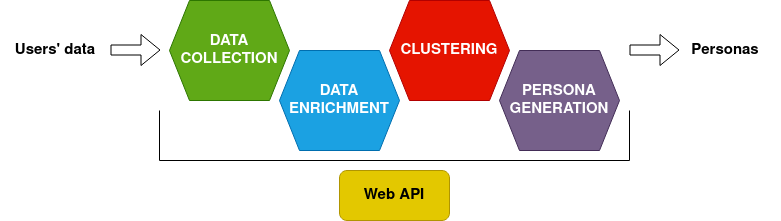
\includegraphics[width=1\textwidth]{img/Pipeline.png}
\caption{High-level view of the main components}
\label{fig:logical_components}
\end{figure}

\subsection{Data collection}
\label{subsec:data_collection}
This component has the task to fetch user data from the web. Since the system should support the creation of personas for many different contexts, the more data can be collected, the better and richer the final personas will be.

The main data source is social media data. While more traditional social networks like Twitter, Facebook or Instagram are supported for the reasons introduced in Chapter \ref{cha:art}, the system is designed to also allow the use of data from less traditional social media (e.g. Strava for sports data, Quora and Medium for user-specific blogging data). To achieve this, a list of all relevant data that can be collected needs to be defined for each data source. Relevant data can include pieces of user information such as name, location, language, number of followers, profile picture and activities (contents the user posted, complete with metadata like the number of likes, comments and shares). It should be noted that different social media usually include different data, which means there could be a lack of data if only one source is used to describe a user. In order to solve this problem, the system allows to associate multiple data sources to a single user.

Another important factor is that user data needs to be periodically collected: in fact, a huge number of activities is posted on social networks every day (around 6000 every second on Twitter\footnote{\url{https://www.dsayce.com/social-media/tweets-day/}}). For this reason, the collection component should run periodically (e.g. every 24 hours) in order to keep user data up to date and to retrieve the latest activities.

In general, this component needs as \textit{input} a series of IDs that identify the user among all the data sources associated to them. The expected \textit{output} is, for each data source, the corresponding user information and \textit{n} user activities. The number \textit{n} of activities to download could be given as a parameter, but it should not be too large in order to avoid overloading the system. For example, Twitter allows to fetch up to 200 tweets per request.

\subsection{Data enrichment}
This component has the task to derive new insights from the data that was previously collected. These insights are what users will ultimately be clustered on, which means that this phase determines how the final personas will look like. The enrichment component is split in two modules: one enriches user activities, and one enriches user profile information.

\subsubsection{Activity enrichment}
\label{subsubsec:activity_enrichment}
The goal of this module is to extract, from activity data (such as raw texts and images) and metadata, useful insights, listed in the table below. While some of them are often directly available from the collected data (such as the language or device used), the biggest challenge is to extract what the activity is about. Such information is important because it allows to gain insights on a user's behavior, such as their interests and personality. This task is further complicated when taking different forms of media (text, images) and different languages into account.

\begin{center}
\begin{tabular}{lll}
\hline
Enrichments & & \\
\hline
\textbf{String} & language & \%Language of the activity (if a text is present) \\
\textbf{Float} & sentiment & \%Value that indicates the tone of the activity \\
\textbf{Set[String]} & entities & \%Strings representing what the user talks about in the activity\\
\textbf{String} & device & \%The device on which the activity was posted \\
\hline
\end{tabular}
\end{center}

The expected \emph{input} is a user activity, as collected in the previous step. The \emph{output} is the enriched activity.

\subsubsection{User profile enrichment}
\label{subsubsec:user_profile_enrichment}
The goal of this module is to make use of whatever data is available from the collected profile information, together with the enriched activities, to extract insights that are relevant for the final personas. For the purpose of designing the system to be as general as possible, we have defined a list of attributes that are present in most persona templates available online: they are shown in the table below. It should be noted that, in many cases, some of the attributes may be impossible to extract: this depends on how much a user is active on a given social media site, and what kind of information they share.

\begin{center}
\begin{tabular}{lll}
\hline
Attributes & & \\
\hline
\textbf{String} & gender & \%Predicted gender \\
\textbf{String} & age & \%Predicted age range (e.g. 19-29) \\
\textbf{String} & type & \%Whether the user profile is of an individual or brand \\
\textbf{String} & location & \%Where the user lives \\
\textbf{String} & prefLanguage & \%The language most used by the user \\
\textbf{String} & maritalStatus & \%Whether the user is single, married, etc. \\
\textbf{Boolean} & hasChildren & \%Whether the user has children or not \\
\textbf{String} & job & \%The profession of the user \\
\textbf{String} & personality & \%Myers-Briggs personality type, encoded in 4 letters \\
\textbf{Set[String]} & interests & \%List of the top interests of the user \\
\textbf{Float} & attitude & \%Average sentiment found in the user's activities \\
\textbf{Dictionary} & activityByTime & \%How much the user is active during each day \\
\textbf{Set[String]} & activeChannels & \%Social channels where the user is most active \\
\hline
\end{tabular}
\end{center}

In order to predict attributes such as gender, age or type, machine learning classifiers can be employed. For example, gender can be predicted from a name, or from a profile picture through the use of computer vision algorithms. Life event detectors could predict a user's marital status and/or if they have children by checking if they have posted about marriage or the birth of a child. Personality can be inferred by how the user interacts with other people (as presented in section \ref{sec:enrichment}), and interests are a result of the entities and topics found in the user's activities.

The expected \emph{input} is the result of the collection of user profile information from a data source and respective enriched activities, while the \emph{output} is the enriched user profile.

\subsection{Clustering}
This component has the task to create clusters of similar users, based on the characteristics that have been extracted in the previous steps. The \emph{input} is a list of users with enriched attributes, and the expected output is composed as follows:
\begin{itemize}
    \item a mapping of each user to the corresponding cluster index;
    \item a list of \textit{representative users}, one for each cluster. A representative user is made up by the characteristics that better define a cluster. It should be noted that it can either be a real user or not, depending on the clustering algorithm. For example, in the K-Means algorithm a representative user would be a \emph{centroid}, which is defined as the average of all the users in a given cluster.
\end{itemize}
The number of clusters that are found could either be specified as a parameter by the user, or could be automatically determined by the system in order to optimize the quality of the clusters.

\subsection{Persona generation}
This component has the task to generate a persona for each cluster defined in the previous step. Since the output of the clustering component includes a list of representative users, this boils down to:
\begin{enumerate}
    \item assign realistic attributes to the representative users, in case they are not directly mapped to real users (e.g. in case a representative user is defined as the average of all users in a given cluster).
    \item give an identity to each representative user: this consists in assigning them a demographically accurate name, photo and textual description.
\end{enumerate}
The \emph{input} is a list of representative users, as output by the clustering component. The \emph{output} is a list of personas, one for each cluster/representative user. Ideally, the user should be able to specify which attributes to include in the personas, in order to tailor them to their specific needs. 

\subsection{Web API}
Users of the service interact with this layer to perform their operations. The main resources are the following:
\begin{itemize}
    \item \textbf{tokens}: they are keys used for authorizing access to protected resources;
    \item \textbf{accounts}: in order to use the service, people need to create an account. This allows them to authenticate for future API requests;
    \item \textbf{brands}: an account can create many brands. A brand is essentially a collection of users: an account can create, for example, a brand for Nutella and a brand for Coca Cola, in order to generate personas independently for the two cases;
    \item \textbf{users}: users are the objects subject to collection, enrichment and clustering. Multiple data sources can be associated to one user. Each user is associated to one and only one brand; the reason behind this is that, if users were shared between brands, an account modifying one of their users (e.g. removing a data source) would have side effects on all the other accounts whose brands include that user;
    \item \textbf{clusters} and \textbf{personas}.
\end{itemize}
In order to prevent unauthorized access to important resources like user data and brand's personas, the resources should be protected. The way in which they are protected is explained in Chapter \ref{cha:implementation}.

\section{Data models}
In this section, the data models used by the system are formalized.

\subsection{Account}
The \texttt{Account} model is composed as follows; other attributes (e.g. name) could be added if needed.
\begin{center}
\begin{tabular}{lll}
\hline
Account & & \\
\hline
\textbf{String} & accountID & \%The unique ID of the account inside the system \\
\textbf{String} & email & \%The email of the user, used for authentication \\
\textbf{String} & hashedPsw & \%Hashed password (with salt), used for authentication \\
\hline
\end{tabular}
\end{center}

\subsection{Brand}
The \texttt{Brand} model is composed as follows:
\begin{center}
\begin{tabular}{lll}
\hline
Brand & & \\
\hline
\textbf{String} & brandID & \%The unique ID of the brand inside the system \\
\textbf{String} & accountID & \%The ID of the account that created the brand \\
\textbf{String} & name & \%The name associated to this brand \\
\hline
\end{tabular}
\end{center}

\subsection{User}
The \texttt{User} model is composed as follows:
\begin{center}
\begin{tabular}{lll}
\hline
User & & \\
\hline
\textbf{String} & userID & \%The unique ID of the user inside the system \\
\textbf{String} & brandID & \%The ID of the brand the user belongs to \\
\textbf{DataSource[]} & dataSources & \%List of data sources associated to the user \\
\textbf{Attributes} & attributes & \%Enriched attributes of the user \\
\hline
\end{tabular}
\end{center}
The \texttt{Attributes} object is described in Section \ref{subsubsec:user_profile_enrichment}. User attributes are populated based on the attributes present in the user's data sources (a merging strategy needs to be defined in case of disagreements between different data sources). 

\subsection{Data Source}
As data sources can be very heterogeneous, a general \texttt{DataSource} object is defined:
\begin{center}
\begin{tabular}{lll}
\hline
DataSource & & \\
\hline
\textbf{String} & sourceID & \%The unique ID of the data source inside the system \\
\textbf{String} & sourceName & \%The name of the data source (e.g. Twitter) \\
\textbf{String} & sourceUserID & \%ID of the user in this specific data source \\
\textbf{String} & username & \%Username of the user in  this specific data source \\
\textbf{String} & from & \%ID of the oldest collected activity of the user \\
\textbf{String} & to & \%ID of the newest collected activity of the user \\
\textbf{Attributes} & attributes & \%Enriched attributes of the user in this specific data source \\
\hline
\end{tabular}
\end{center}
Then, for each particular data source that is supported, a specific object needs to be defined. For example, a \texttt{TwitterDataSource} would contain the general \texttt{DataSource} properties, plus additional ones, such as: name, location, profile image, description, website, number of followers and following.

\subsection{Activity}
The same considerations about data sources heterogeneity apply to activities. A general \texttt{Activity} model is composed as follows:
\begin{center}
\begin{tabular}{lll}
\hline
Activity & & \\
\hline
\textbf{String} & activityID & \%The unique ID of the activity inside the system \\
\textbf{String} & sourceName & \%The name of the data source where the activity is from \\
\textbf{String} & sourceUserID & \%ID of the activity in this specific data source \\
\textbf{String} & authorID & \%ID of the user (in this data source) who posted the activity \\
\textbf{Enrichments} & enrichments & \%Enriched activity properties\\
\hline
\end{tabular}
\end{center}
where the \texttt{Enrichments} model is  the one described in Section \ref{subsubsec:activity_enrichment}. A more specific \texttt{TwitterActivity} would contain additional properties, like: text, language, media, hashtags, external links, number of likes and shares.

\subsection{Cluster}
The \texttt{Cluster} model is composed as follows:
\begin{center}
\begin{tabular}{lll}
\hline
Cluster & & \\
\hline
\textbf{String} & clusterID & \%The unique ID of the cluster inside the system \\
\textbf{String} & brandID & \%The ID of the brand the cluster belongs to \\
\textbf{User[]} & users & \%List of users who belong to the cluster \\
\textbf{Attributes} & representative & \%Attributes of a user who represents the cluster \\
\hline
\end{tabular}
\end{center}

\subsection{Persona}
The \texttt{Persona} model is composed as follows:
\begin{center}
\begin{tabular}{lll}
\hline
Persona & & \\
\hline
\textbf{String} & personaID & \%The unique ID of the persona inside the system \\
\textbf{String} & clusterID & \%The ID of the cluster the persona represents \\
\textbf{String} & name & \%Name of the persona \\
\textbf{String} & photo & \%Photo of the persona \\
\textbf{String} & description & \%Brief textual description of the persona \\
\textbf{Attributes} & attributes & \%Attributes of the persona \\
\hline
\end{tabular}
\end{center}

\section{System architecture}
A diagram of the system architecture is shown in Figure \ref{fig:architecture}.

The system can be logically divided in two macro-components: the first contains the collection and enrichment components, the second contains the clustering and persona generation ones. The former is described in Section \ref{subsec:pub/sub}, due to its complexity .

The latter is less complex, since it mostly works with internal data. Each clustering (and persona generation) request is fulfilled with whatever data is available at the moment. First, clusters are generated; after that, they are passed, together with representative users, to the persona generation module. This macro-component should also be able to run periodically (e.g. every 30 minutes), in order to always keep personas updated when new user data is collected.

\begin{figure}
\centering
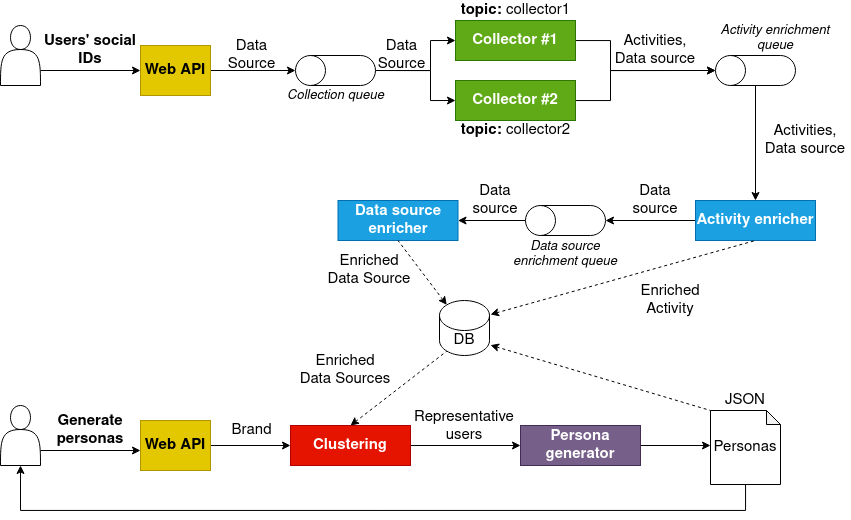
\includegraphics[width=\textwidth]{img/Architecture.png}
\caption{System architecture}
\label{fig:architecture}
\end{figure}

\subsection{Pub/Sub system for Collection and Enrichment}
\label{subsec:pub/sub}
A stream-processing design was chosen for our system. The reasons behind this choice are the following: first of all, social network data naturally falls under the category of \emph{real time data}. As mentioned in Section \ref{subsec:data_collection}, a huge number of data is posted on social networks every second, and the system would quickly get overloaded if high quantities of user data is processed in batches. Additionally, the system achieves high separation of concerns: this means that each module does not need to care about the status of other modules, and only needs to carry out its task. This also allows for the implementation of atomic, simple modules and makes the system more easily scalable and expandable, for example, in case support for a new social network needs to be added.
 
A \emph{pub/sub} (publisher/subscriber) system is one way to achieve the previously mentioned design. It consists in queues that allow communication between each module. A module can publish any kind of message on a queue with a given \emph{topic}, and all the modules that \emph{subscribed} to that topic receive the message. When one module is busy, all the incoming messages are queued and wait until they are taken by the module to be processed.

As an example, let us suppose that a user with two data sources is created through the web API: a Twitter and Facebook account. After saving the user in a database, the user ID on Twitter and Facebook are published on the \emph{collection queue}: the former is published under the topic \emph{twitter}, the latter under the topic \emph{facebook}. The Twitter and Facebook collector modules are always active, listening on the queue for their respective topics. Once the user IDs are received, the two modules independently download data, save it into the database, and publish the newly collected activities on another queue, the \emph{activity enrichment queue}. Activities are enriched, saved into the database, and once all activities of a given data source have been enriched, the data source is sent to the \emph{data source enrichment queue}. Finally, data sources are enriched and saved into the database.
      \NewPage
      \chapter{Implementation}
\label{cha:implementation}
In this chapter, the implementation of a prototype of the system is presented. Due to time constraints and the overall complexity of the system, some features that are presented in Chapter \ref{cha:design} are not implemented in the final prototype. They mostly consist of individual classifiers to enrich user data such as marital status or number of children, which ultimately do not impact the larger structure and functionality of the system. In fact, this can be seen as proof that the system design meets the requirement of being highly customizable and expandable.

The whole prototype is developed in Python, one of the most complete programming languages when it comes to the availability of machine learning and other user-made libraries. Every component presented in the design section consists in a separate package. In the sections below, those components are described in more detail one by one: the implementation choices for the database and the pub/sub system; how data is collected only from Twitter due to privacy reasons; how the enrichments are performed and what kind of external tools are used for that purpose; what clustering algorithm is used and why; what tools are used to assign an identity to personas; and how the web API was implemented and what functionalities in particular it provides. Finally, a section is dedicated to showing the typical flow of actions and data through the system, in order to understand how all components interact with each other.

\section{Database}
Given the unstructured nature of the data that the system handles, a non-relational database was chosen. In particular, the choice fell on \texttt{Redis}\footnote{\url{www.redis.io}}, an open source, in-memory data structure store that can be used both as a database, cache and message broker. By working in-memory, it can achieve high performance over traditional databases. Data is stored in key/value pairs, as in a typical dictionary data structure: keys are always strings, while values can be a range of supported data types. For our use-case, since complex, nested data models need to be stored, we installed \texttt{RedisJSON}\footnote{\url{www.redislabs.com/blog/redis-as-a-json-store}}, a module that adds support for a JSON data type. This means that all models are converted to and from JSON every time they need to be stored or retrieved from the database. The database runs in a dedicated Docker container.

\section{Pub/Sub}
The Pub/Sub queue system is implemented with the MQTT protocol. The implementation provided in the library \texttt{paho-mqtt}\footnote{\url{www.eclipse.org/paho/}} is used. All the messages are sent and received with a \emph{Quality of Service} (QoS) level of 1, which guarantees that every message is delivered at least once. This allows for the modules that disconnect for any reason to recover all not-received messages once they go back online.

\section{Data collection}
\label{sec:data_collection_imp}
The data source on which the prototype is based is Twitter. Facebook products (such as Facebook itself and Instagram) were considered, but developing an application that works with them has become difficult due to strict privacy policies. In fact, in order to collect data of a user through their API, it is first needed to get explicit authorization of the user. Finding enough users available to share their data for the development of this system would have been a lengthy process. Also other services were taken into consideration, but were ultimately scrapped due to a lack of an API or the unavailability of a free version of the latter.

In order to use the Twitter API, it is first needed to submit a request explaining what you are going to use the API and the collected data for. After confirmation, the API provides a free plan, although with some restrictions on the rate at which requests are made (e.g. 1500 requests every 15 minutes to retrieve tweets). The free plan allows us to get all the information that is needed: user profile information and user tweets. The API is accessed using the \texttt{tweepy}\footnote{\url{www.tweepy.org}} library, which provides a convenience class that handles requests and parameters. It also handles rate limitations by suspending the process until a new time slot is available.

\section{Data enrichment}
This component is divided in two smaller modules that are run independently: one to enrich activities, and one to enrich data sources. They are presented in the sections below.

\subsection{Activity enrichment}
The main task of this module is to extract \emph{language}, \emph{sentiment} and \emph{entities} from an activity, which can contain text and/or images.

An \emph{entity} is a person, an object or a concept that has an article on Wikipedia; for example, the phrase \textit{"I'm studying computer science at the university"} has two entities - \texttt{Computer science} and \texttt{University}. Entity extraction is a powerful approach to figure out what a user talks about in an activity: it supports both texts and images, and it is expandable to many languages (it is only needed, for example, to convert entities, which are Wikipedia articles, to their English article counterpart).

While there exist tools that allow entity extraction from images, such as the \texttt{Cloud Vision API} of Google Cloud\footnote{\url{cloud.google.com/vision}}, they were not used in the prototype due to their heavily restricted free plans. This limits the prototype to only work with texts, but, in a production environment, support for images could greatly improve the accuracy of the final results, since many social media posts don't include any text.

For all three enrichments, we used an external semantic analyzer called \texttt{Dandelion}\footnote{\url{dandelion.eu}}, developed by Spazio Dati\footnote{\url{spaziodati.eu/it}}. It works by using Wikipedia pages as entities, as explained in Section \ref{subsubsec:activity_enrichment}. It provides useful options to optimize entity extraction from short texts coming from social networks, which makes it adequate for our use-case. Additionally, it supports a total of 50 languages, 43 of which are in beta support. The free plan allows the use of 1000 credits per day, and 2.1 credits are used for enriching each activity. This means that only 476 activities can be enriched per day for free. U-Hopper provided a token with 10000 credits, which allows to enrich ten times that amount.

\subsection{Data source enrichment}
This module has the task of enriching the \texttt{Attributes} properties detailed in Section \ref{subsubsec:user_profile_enrichment}.

\textbf{Gender}, \textbf{age} and \textbf{type} are predicted based on the profile image of a user on a given data source. A customized version of the \texttt{M3-Inference}\footnote{\url{github.com/euagendas/m3inference}} library is used for this purpose. Since predicting an exact age is too difficult, four age brackets are given as possible output: $\leq$18, 19-29, 30-39, $\geq$40. In case a profile image is not available, an external API called \texttt{NamSor}\footnote{\url{www.namsor.com}} is used to predict gender and type from a first or full name. This is not always reliable, since the name field is free form on Twitter, which means that a user can choose a fictional name (as opposed to Facebook, which enforces the use of real names).

The \textbf{preferred language} is chosen by keeping a map between all the languages the user has used in their activities, and how many times each language is used. The preferred language is therefore the most used language throughout all activities.

\textbf{Attitude} is simply computed as the average of all sentiment scores found in the user's activities, while \textbf{interests} are more complex to extract. First, the system keeps track of an \emph{entity map} for each data source; it consists in a dictionary where the keys are the entities found in the user's activities, and the values are how many times that entity was found. This is then given as input to a Tapoi model, proprietary of U-Hopper, which functions as follows:
\begin{enumerate}
    \item the model is defined by a fixed set of categories of interest, which represent the full set of interests that are expected as output. Those categories are represented by Wikipedia pages, and in our case are the following: \texttt{Arts, Filmmaking, Cooking, Culture, Economy, Entertainment, Fashion, Geography, Health, History, Literature, Music, Nature, Philosophy, Po\-li\-tics, Religion, Science, Sports, Technology};
    \item the model traverses the Wikipedia graph upwards, starting from each entity found in the entity map, for a fixed number of steps (usually 5);
    \item each time a category of interest is found while traversing the graph, a score is added to that category, proportional to the number of times the respective entity is found in the entity map;
    \item the output is a mapping between each category of interest and their respective scores, which are in the $[0,1]$ range. All scores sum up to 1, and a high score means that the user is interested in the corresponding category.
\end{enumerate}

Two Tapoi models were made available by U-Hopper for this thesis: one that works on English Wikipedia, and one on Italian Wikipedia. While it is possible to use both models for analyzing English and Italian activities, this would mean supporting only two languages. The implemented solution, instead, only uses the English model: if an entity is in another language, it first gets converted to the respective English page on Wikipedia (when available) through the MediaWiki API\footnote{\url{www.mediawiki.org/wiki/API:Main_page}}. The English model was chosen over the Italian one due to English Wikipedia having the largest number of articles than any other language.

As for the rest of the \texttt{Attributes}, they are not implemented due to time constraints, but other Tapoi models exist to predict many of them.

\section{Clustering}
The most important implementation choices for this component are: the features on which to perform clustering; the choice of a distance metric, needed to compute how similar (or dissimilar) two users are; and the actual clustering algorithm. The order in which those implementation choices are listed is not casual: the choice of algorithm depends on the distance metric, and the distance metric depends on what types of features are used.

\subsection{Features}
The chosen features are the \texttt{Attributes} properties that are implemented, minus the type; that is: gender, age, preferred language, attitude and interests. The type is excluded because we decided to deal only with users who are classified as "humans", since personas are ultimately fictional individuals. The features are a mix of \emph{nominal}, \emph{ordinal} and \emph{numerical} data:
\begin{itemize}
    \item nominal data is data that takes on discrete values and does not possess a meaningful order. In our case, gender and preferred language fall under this category;
    \item ordinal data is data that takes on discrete values but possesses a meaningful order. Age is an example of this: it can take on three different values ($\leq$18, 19-29, 30-39, $\geq$40), and it makes sense to say that the bracket $\leq$18 is closer to 19-29 than it is to 30-39;
    \item numerical data is data that takes on continuous values. Attitude is an example, as it is a decimal number in the range $[0,1]$.
\end{itemize}
Interests do not fall directly into any category, but are closer to a mix of nominal data (interest labels) and numerical data (scores).

\subsection{Distance metric}
\label{subsec:distance_metric}
Since we are dealing with mixed data, the most commonly used distance metric, euclidean distance, cannot be used, as it only works with numerical data. This also locks out the choice of K-Means as the clustering algorithm, since it relies on the concept of mean, which is only meaningful in a continuous space. The chosen distance metric is therefore the \emph{Gower distance}, which supports mixed data~\cite{tuerhong2014gower}. It is defined as follows:
\begin{equation*}
    D_{Gower}(x_1,x_2)=\frac{1}{p}\sum_{j=1}^{p}d_j(x_{1j},x_{2j})
\end{equation*}

In words, it is computed as the average of partial dissimilarities across objects with $p$ features. A partial dissimilarity $d_j$ is computed between two objects $x_1$ and $x_2$ on a particular feature $j$, and depends on the type of the feature (ordinal, numerical or nominal):
\begin{equation*}
    \begin{split}
        d_{j,ord}(x_1,x_2)=\frac{\lvert rank(x_{1j})-rank(x_{2j})\rvert}{range_j}
    \end{split}
    \qquad
    \begin{split}
        d_{j,num}(x_1,x_2)=\frac{\lvert x_{1j}-x_{2j}\rvert}{range_j}
    \end{split}
    \end{equation*}
    \begin{equation*}
        d_{j,nom}(x_1,x_2)=
        \begin{cases}
            1 & \text{if}\ x_{1j}\neq x_{2j} \\
            0 & \text{otherwise}
        \end{cases}
\end{equation*}
where $rank(x_j)$ is the ordinal number assigned to feature $x_j$, and $range(j)$ is defined as the difference between the maximum and minimum values of feature $j$.

A modified version of the Gower distance is used in our system: instead of simply averaging all partial dissimilarities, a weighted average is computed. This allows to give more weight to features that can be considered more important, like the interests in our case.

\subsection{Clustering algorithm}
Since we have defined a custom distance metric, only algorithms that support either a distance function as a parameter or a precomputed distance matrix can be chosen. Given $n$ users, we define a distance matrix $M[n\times n]$, where each cell $M[i,j]$ contains the distance between user $i$ and user $j$.

The chosen algorithm is called \emph{K-Medoids}\footnote{\url{en.wikipedia.org/wiki/K-medoids}}, an alternative version of K-Means that accepts a precomputed distance matrix as an input parameter. Instead of computing a centroid as the mean of all objects in a cluster, the algorithm chooses a medoid; it can be defined as the object of a cluster whose average dissimilarity to all the other objects of the cluster is minimal, that is, the most centrally located point in the cluster. Using K-Medoids also has the advantage that medoids, as opposed to centroids, are real data points (i.e. users), which means that they can be directly given as input to the persona generation component.

The main challenge remains deciding the right number $k$ of clusters, which needs to be specified a priori. The chosen way is trying models with different values of $k$, ranging from 2 to 10, since we do not want a large number of clusters. For each model, we compute the average \emph{silhuette score}\footnote{\url{en.wikipedia.org/wiki/Silhouette_(clustering)}}: it is a number between -1 and 1 which measures how similar an object is to its own cluster (cohesion) compared to other clusters (separation). The optimal number of clusters is therefore the one that maximizes the average silhuette score.

\section{Persona generation}
This component is simpler than the others, especially since the clustering algorithm outputs representative users with meaningful attributes. Given a representative user, it is needed to enrich it with a name, photo and textual description.

The \textbf{name} is generated through an external API called \texttt{Name Parser}\footnote{\url{parser.name}}. It allows to optionally specify a gender and a country, in order to get demographically accurate names.

The \textbf{photo} is taken from a predefined set of photos; for the purpose of the prototype, the set is composed of five photos for each gender and age bracket, for a total of 40 photos. The photos were taken manually through a website\footnote{\url{thispersondoesnotexist.com}} that uses AI to generate pictures of people that do not exist.

The \textbf{description} was not implemented due to time constraints, but a valid approach would be to write one or more templates that can be appropriately filled with the persona attributes.

\section{Web API}
The web API is implemented using the \texttt{Flask}\footnote{\url{flask.palletsprojects.com/en/2.0.x/}} framework, extended with the \texttt{Flask-RESTful} library. The chosen method for managing authentication and authorization is a JWT Token, a particular implementation of token/bearer authentication. Each token contains the ID number of the account that generated the token, and it is checked in order to grant or deny access to a requested resource. It also contains an expiration date, after which the token is no longer valid. In the prototype, like is often seen in web APIs, the expiration date is not set; this means that it is up to the user of the service to keep the token secret. In any case, it is possible to regenerate a token, a process which invalidates the previous one.

Figure \ref{fig:api_funcs} shows the main functionalities provided by the web API (the lock icons show what resources need authorization). The complete specification and documentation is available at the link below:
\begin{center}
\url{app.swaggerhub.com/apis-docs/nicola-farina/personas/1.0.0}
\end{center}

\begin{figure}[h]
\centering
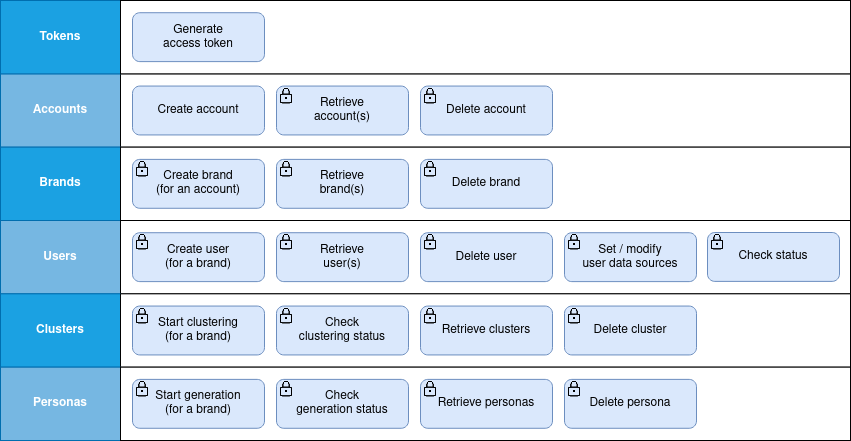
\includegraphics[width=1\textwidth]{img/APIfuncs.png}
\caption{Functionalities provided by the API}
\label{fig:api_funcs}
\end{figure}

\section{Flow of the system}
Figure \ref{fig:enrichment_flow} shows a typical flow of the data collection and enrichment components in detail, while Figure \ref{fig:flow} shows the flow of the whole system. 

The implementation of the collection and enrichment components takes the advantages of real time data processing while still allowing to keep track of progress. In order to do so, a \texttt{Computation} object is created whenever a process of data collection and enrichment begins: it is simply composed by a unique ID and a \emph{status} field. Those objects are stored in the database, and every 24 hours all computation objects whose value equals \emph{done} are deleted, since they are no longer needed. Another advantage of keeping track of the progress is that data sources can be sent for enrichment only when all related activities are enriched. This is preferable because, if there was no way to keep track of how many activities have been enriched, data sources would have to be enriched after every single activity. This would result in a lot of external API calls, which may have severe rate limitations.

\begin{figure}[h!]
\centering
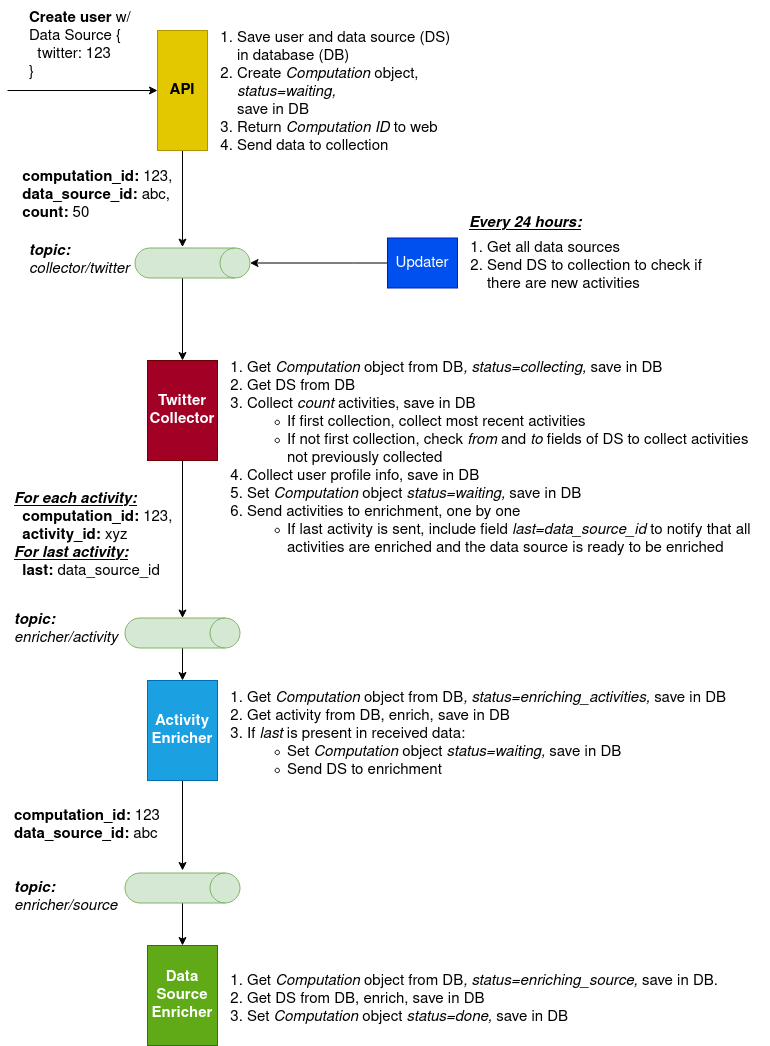
\includegraphics[width=0.95\textwidth]{img/EnrichmentFlow.png}
\caption{Detailed flow of collection and enrichment components}
\label{fig:enrichment_flow}
\end{figure}

\begin{figure}
\centering
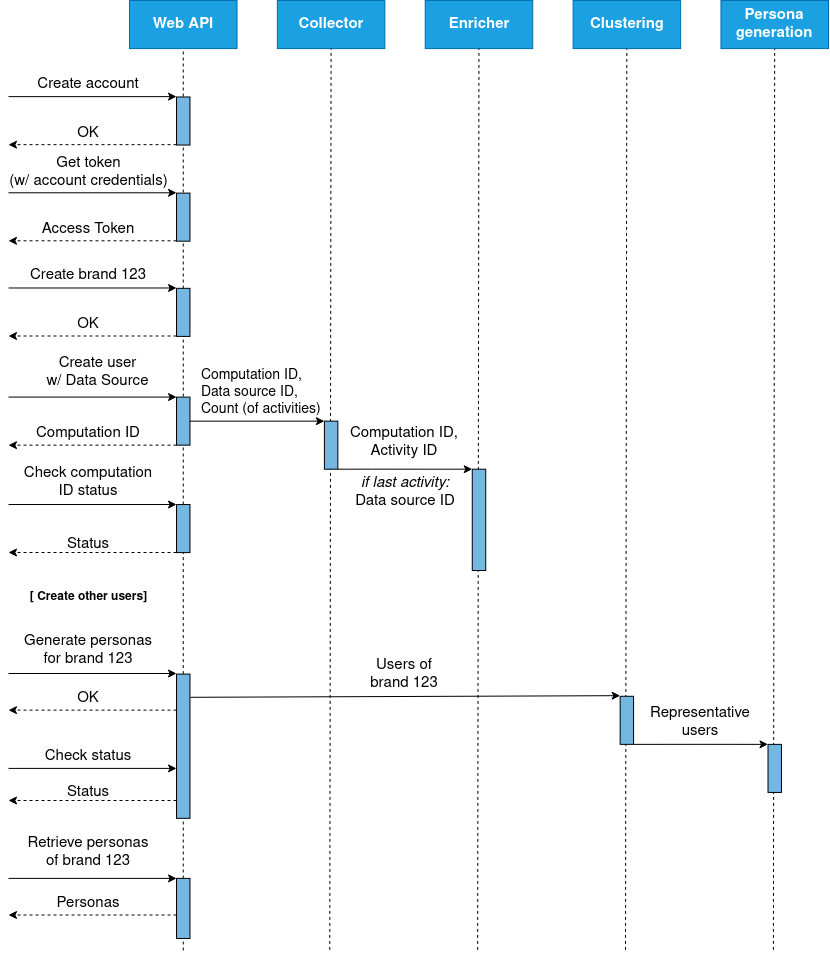
\includegraphics[width=\textwidth]{img/SystemFlow.png}
\caption{Typical flow of actions and data in the system}
\label{fig:flow}
\end{figure}

      \NewPage
      \chapter{Evaluation}
\label{cha:evaluation}
In this chapter, the evaluation of the implemented prototype is presented. First, the different evaluation metrics and experiments are discussed. Then, the test dataset is described. Finally, the experiments and their results are analyzed.

\section{Evaluation metrics}
Two main factors are taken into consideration for evaluating the prototype: the quality of the clusters, which directly translates into the quality of the personas; and the performance.

\subsection{Quality of clusters}
With quality of a cluster we mean how coherent a cluster, both within itself (\textit{are the users of a cluster similar?}) and with all the users that were clustered (\textit{if there are football players among them, a cluster of sports enthusiast should be expected}). This depends on the number of clusters chosen a priori, on the distance metric and on the minimum number of activities that are collected for each user. The number of activities is relevant because, if it is too low, the chance of users' interests being misclassified in the enrichment part gets higher, since the impact of outlying activities is stronger. 

Evaluating the quality of a cluster is not an easy task, since clustering falls under the category of \textit{unsupervised learning}. This means that, usually, there is no ground truth that allows to check whether the clustering result is good or not. In fact, oftentimes the results are analyzed manually. This approach is not feasible for our fully deployed system, since the requirement of full automation would not be met. For this reason, and for the purpose of evaluation, we manually labeled our testing dataset with ground truths. This allows us to use four classic machine learning metrics, which range from 0 to 1, with 1 being the best score:
\begin{equation*}
    \begin{split}
        Accuracy = \frac{TP + TN}{TP + TN + FP + FN}
    \end{split}
    \quad
    \begin{split}
        Precision = \frac{TP}{TP + FP}
    \end{split}
    \quad
    \begin{split}
        Recall = \frac{TP}{TP + FN}
    \end{split}
\end{equation*}
where TP means \textit{true positives}, TN \textit{true negatives}, FP \textit{false positives} and FN \textit{false negatives}.
\subsection{Performance}
For performance, relevant metrics are the average time needed to enrich a single source or a single activity, as well as the total time needed for the entire process of generating personas from a collection of users.

\section{Test dataset}
The test dataset was built manually in order to have accurate ground truths. For this reason, and due to time constraints (further enforced by the APIs rate limitations), it is only composed of 90 users.

Those 90 users are all public figures who have a profile on Twitter, and were chosen in the following way: 30 football players, 30 politicians and 30 musicians/singers. These categories can be mapped to the interests classified by our system: respectively, \textit{sports}, \textit{politics} and \textit{music}. Of course, not every tweet of a politician is about politic. This was taken into account during the creation of the dataset, and only users who mainly tweeted about their respective categories were chosen.

As mentioned previously, each user is assigned a ground truth: their gender, their age bracket and their main field of interest (sports, politics, music).

\section{Experiments setup}
We have identified a set of tests, in order to evaluate the key features of the prototype. They are shown in Table \ref{table:experiments}.

In \texttt{Test1} and \texttt{Test2}, the time it takes to enrich activities and data sources is computed. \texttt{Test3} is the most important test, in which the quality of the clusters is computed and the effects of parameters like the distance metric, the number of clusters and the number of activities per user are analyzed.

\begin{table}[h]
\centering
\begin{tabular}{|c|c|c|}
    \hline
    & \textbf{Operation} & \textbf{\# of activities per user} \\
    \hline
    Test1 & Activities enrichment & [20, 50, 100] \\
    \hline
    Test2 & Data sources enrichment & [20, 50, 100] \\
    \hline
    Test3 & Clustering & [20, 50, 100] \\
    \hline
\end{tabular}
\caption{Experiments}
\label{table:experiments}
\end{table}

Other tests, for example, to evaluate the quality of the individual classifiers used in the enrichment process, are left out due to time constraints.

\section{Evaluation results}

\subsection{Activities enrichment}
The results are shown in Table \ref{table:activity_time}. As expected, the time to enrich a single activity is more or less constant. It is computed as the time difference between the reception of the activity on the enrichment queue and the moment the enriched activity is saved in the database. This average is, as expected, not influenced by the number of activities collected per user, since each enrichment is independent from the others. It is only influenced by the external API call and the time it takes to save the enrichments in the database.

The total time to enrich a given number of activities for each of the 90 users is not simply the number of total activities multiplied by the time it takes to enrich a single activity. This is caused by the quality of service setting of the pub/sub queue: by having it set to one, more time is required since the messages needs to be acknowledged before they can be processed. We have not tried setting it to zero, since some queue clients seem to disconnect at times, and that would mean losing all the messages that are sent while a client is offline. It is worth noting how, in order to collect 100 activities, the system needs to wait an entire day; this is because of the activity enrichment API, which allows at most 4500 activities to be fully enriched per day.

\begin{table}[h]
\centering
\begin{tabular}{|c|c|}
    \hline
    \textbf{Operation} & \textbf{Elapsed time} \\
    \hline
    Single activity & 0.52 seconds (average) \\
    \hline
    20 activities per 90 users & 16 minutes \\
    \hline
    50 activities per 90 users & 36 minutes \\
    \hline
    100 activities per 90 users & 75 minutes + 24h wait \\
    \hline
\end{tabular}
\caption{Performance results for activity enrichment}
\label{table:activity_time}
\end{table}

\subsection{Data sources enrichment}
The time to enrich a single data source sits at an average of 13,5 seconds, and is dominated by the interests classifier. As expected, the total time to enrich a data source is practically not affected by the number of activities per user, since the only thing that changes is the number of activities that need to be retrieved from the database. The total time to enrich 90 users is around 20 minutes.

\subsection{Clustering}
\subsubsection{Distance metric}
The distance metric used for clustering is specified in Section \ref{subsec:distance_metric}. The only parameters that needed tuning are the weights assigned to each feature. The weights were tuned in order to maximize the quality of the clusters that are presented in the following sections. Furthermore, a lot of importance was given mostly to interests, followed by gender, based on the fact that interests are the most relevant behavioral attributes available in our case for defining personas. The weights are the following:
\begin{gather*}
    Gender = 0.5 \quad Age = 0.5 \quad Language = 0.3 \quad Interests = 13 \quad Attitude = 0.3
\end{gather*}
While the weight for interests may seem high, based on tuning and experiments we conducted, it only begins to suppress the other weights around the value 100. If lowered, the gender feature tends to dominate, resulting most of the times in only two clusters, one for males and one for females.

\subsubsection{Number of clusters and activities per user}
Figure \ref{fig:silhuette} shows the silhuette score for various number of clusters and for the three different values of activities per user. It is clear that going from 20 to 50 activities per user helps narrow down the main interests of a user, thus reducing the optimal number of clusters from ten to four. Going from 50 to 100 activities does not change much, so we chose 50 as the optimal number of activities per user, which also avoids having to wait one day due to API rate limitations.

Why this happens is that, if only a small number of activities are analyzed, the risk of misclassifying a user’s interests is high. For example, during the period when our dataset was created, many Italian users tweeted about the UEFA European Football Championship, even politicians and singers. One way to avoid classifying users based on outlying activities is to simply increase the number of activities per user, thus decreasing the impact of outliers. A more sophisticated approach would consist in keeping track of what the users talk about over time, for example, month by month. This way, interests that are present only for a limited amount of time could be classified as outliers, and left out of the overall interests of the user.

\begin{figure}[h]
\centering
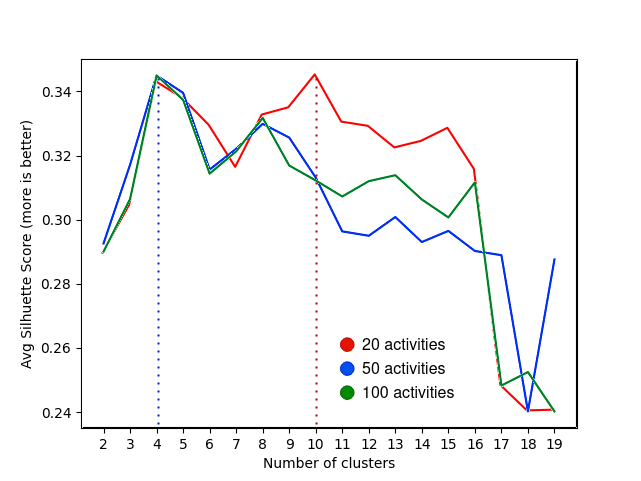
\includegraphics[width=0.65\textwidth]{img/Silhuette.png}
\caption{Silhuette score for each number of clusters, for different values of activities per user}
\label{fig:silhuette}
\end{figure}

\subsubsection{Composition of each cluster}
At this point, we analyzed how each cluster is composed. Table \ref{table:repr_users} shows the representative users, and we assigned a name to every cluster based on them. Table \ref{table:summary_clusters} shows data that can be used for computing precision, recall and accuracy.

At first glance, the results seem to be coherent with the ground truth. Two things should be noted: the first is that only musicians were split in two clusters based on gender (while the other categories are left with mixed genders); the second is that all of the representative users have \emph{culture} as their second main interest. This last observation probably happens due to the very general scope of a category such as culture. This issue could be solved by using more specialized interests classifiers, which could be chosen as a parameter by the user in order to obtain more accurate results for a specific sector (e.g. there could be one classifier specialized for the music industry, one for sports, one for food etc.). Another approach to solve it would be to ignore a specific interest if it shows up in the majority of the clusters.

\begin{table}[]
\centering
\begin{tabular}{|c|c|c|c|c|c|}
    \hline
    \textbf{Cluster} & \textbf{Gender} & \textbf{Age} & \textbf{Pref. lang.} & \textbf{Top 2 interests} & \textbf{Attitude} \\
    \hline
    1, Politicians & male & $\geq 40$ & it & Politics (0.35), Culture (0.16) & 0.02 \\
    \hline
    2, Musicians (F) & female & 19-29 & en & Music (0.26), Culture (0.10) & 0.36 \\
    \hline
    3, Musicians (M) & male & $\geq 40$ & en & Music (0.49), Culture (0.16) & 0.13 \\
    \hline
    4, Footballers & male & 30-39 & it & Sports (0.62), Culture (0.08) & 0.12 \\
    \hline
\end{tabular}
\caption{Representative users of each cluster}
\label{table:repr_users}
\end{table}

\begin{table}[]
\centering
\begin{tabular}{|c|c|c|c|c|c|}
    \hline
    \textbf{Cluster} & \textbf{\# of users} & \textbf{\# of expected users} & \textbf{TP} & \textbf{FP} & \textbf{FN}\\
    \hline
    1, Politicians & 31 & 30 & 29 & 2 & 1\\
    \hline
    2, Musicians (F) & 17 & 15 & 15 & 2 & 0 \\
    \hline
    3, Musicians (M) & 13 & 15 & 13 & 0 & 2 \\
    \hline
    4, Footballers & 29 & 30 & 29 & 0 & 1 \\
    \hline
\end{tabular}
\caption{Summary of the contents of each cluster}
\label{table:summary_clusters}
\end{table}

With this data, we can compute the metrics introduced earlier in this chapter to assess the quality of the clusters: they are shown in Table \ref{table:results}.

\begin{table}[h]
\centering
\begin{tabular}{|c|c|c|c|}
    \hline
    \textbf{Cluster} & \textbf{Accuracy} & \textbf{Precision} & \textbf{Recall} \\
    \hline
    1, Politicians & 0.96 & 0.93 & 0.96 \\
    \hline
    2, Musicians (F) & 0.97 & 0.88 & 1.0 \\
    \hline
    3, Musicians (M) & 0.97 & 1.0 & 0.86 \\
    \hline
    4, Footballers & 0.98 & 1.0 & 0.96 \\
    \hline
    Global (average) & 0.97 & 0.95 & 0.94 \\
    \hline
\end{tabular}
\caption{Results of clustering}
\label{table:results}
\end{table}

While the results are very positive, it should be noted that there is the possibility of \emph{overfitting}: that means that the system performs well on this specific test dataset, but does not generalize enough to perform well on other datasets. The only way to find out if this is the case is to try to evaluate the system with other datasets, for example by adding other categories of users. This is left out of this thesis due to time constraints.

\subsection{Final considerations}
The results of the clustering evaluation directly reflect the quality of the personas. In fact, almost all users in our dataset fall under a cluster that represents them, and the clusters themselves are meaningful and can be given an identity.

As for evaluating the personas themselves, this is still an open issue that is currently being researched. This is the case because there currently are no ways to algorithmically (thus, automatically) evaluate the quality of a persona profile; the current, most employed solution simply consists in handing out the personas to a marketing specialist, who is able to judge whether they could be useful for defining marketing strategies and choices. Again, this part is not covered in this thesis due to time constraints.
      \newpage
      \chapter{Conclusions}
\label{cha:conclusions}
This thesis tries to answer the research question about the feasibility of automatic persona generation from social media data, proposing a solution that is scalable and expandable to multiple social media, and presenting a prototype that works with Twitter data.

It develops on what is the current state of the art, especially because it is one of the only works that discusses in depth about all the phases of the process, and does not focus only on clustering. The enrichment component makes use of innovative techniques, such as using Wikipedia contents to understand what a user talks about, which allows to support a large number of languages and to use all components of an activity (text, images, but also external links etc.) for classification purposes. The proposed system architecture and data models are for general purpose personas, but they are designed to allow the creation of sector-specific personas by introducing new classifiers. Furthermore, the stream processing design allows to avoid bottlenecks as much as possible and achieves a high separation of concerns.

The system shows great results, with clustering accuracy, precision and recall measures well above 0.9, as well as high accuracy enrichments.

While many features were not implemented in the final prototype, either due to time constraints or privacy reasons, this work offers a solid base for automatically generating marketing personas from social media data, which can be deepened in some aspects based on the specific scope in which it will be used.

\section{Future work}
There are several aspects that can be deepened or added. First of all, the system was designed to work with several social networks and similar sites in mind, but due to the reasons explained in Section \ref{sec:data_collection_imp} only Twitter was taken into consideration for the prototype. The first logical addition would be to add support for other social networks: first of all, Facebook would be a good choice, since it is a great source of personal information and demographics that are hard to come by on Twitter.

Another important improvement would be adding enrichment modules to predict all the attributes that were not considered in the prototype due to time constraints. Information such as location, marital status and personality would add great value to the final personas. The same applies for personas themselves: implementing a textual description for each of them would add a lot of value to their use.

More time could be spent on the evaluation of the clusters and on fine-tuning parameters such as the distance metric weights. Testing the system on a dataset with a lot more than 90 users would provide more accurate results, and possibly confirm or rule out the possibility of overfitting.

Making use of sector-specific classifiers would also greatly improve the quality of personas for non-general use cases.

Finally, providing a web application with a graphical interface to use the service would be an important addition to provide a better user experience and simplify the interactions. It would also allow to visualize personas with nice graphics, which is how they are usually presented to marketing specialists.

      \NewPage
      
    \endgroup


    % bibliografia in formato bibtex
    %
    % aggiunta del capitolo nell'indice
    \addcontentsline{toc}{chapter}{Bibliography}
    % stile con ordinamento alfabetico in funzione degli autori
    \bibliographystyle{plain}
    \bibliography{biblio}
%%%%%%%%%%%%%%%%%%%%%%%%%%%%%%%%%%%%%%%%%%%%%%%%%%%%%%%%%%%%%%%%%%%%%%%%%%
%%%%%%%%%%%%%%%%%%%%%%%%%%%%%%%%%%%%%%%%%%%%%%%%%%%%%%%%%%%%%%%%%%%%%%%%%%
%% Nota
%%%%%%%%%%%%%%%%%%%%%%%%%%%%%%%%%%%%%%%%%%%%%%%%%%%%%%%%%%%%%%%%%%%%%%%%%%
%% Nella bibliografia devono essere riportati tutte le fonti consultate 
%% per lo svolgimento della tesi. La bibliografia deve essere redatta 
%% in ordine alfabetico sul cognome del primo autore. 
%% 
%% La forma della citazione bibliografica va inserita secondo la fonte utilizzata:
%% 
%% LIBRI
%% Cognome e iniziale del nome autore/autori, la data di edizione, titolo, casa editrice, eventuale numero dell’edizione. 
%% 
%% ARTICOLI DI RIVISTA
%% Cognome e iniziale del nome autore/autori, titolo articolo, titolo rivista, volume, numero, numero di pagine.
%% 
%% ARTICOLI DI CONFERENZA
%% Cognome e iniziale del nome autore/autori (anno), titolo articolo, titolo conferenza, luogo della conferenza (città e paese), date della conferenza, numero di pagine. 
%% 
%% SITOGRAFIA
%% La sitografia contiene un elenco di indirizzi Web consultati e disposti in ordine alfabetico. 
%% E’ necessario:
%%   Copiare la URL (l’indirizzo web) specifica della pagina consultata
%%   Se disponibile, indicare il cognome e nome dell’autore, il titolo ed eventuale sottotitolo del testo
%%   Se disponibile, inserire la data di ultima consultazione della risorsa (gg/mm/aaaa).    
%%%%%%%%%%%%%%%%%%%%%%%%%%%%%%%%%%%%%%%%%%%%%%%%%%%%%%%%%%%%%%%%%%%%%%%%%%
%%%%%%%%%%%%%%%%%%%%%%%%%%%%%%%%%%%%%%%%%%%%%%%%%%%%%%%%%%%%%%%%%%%%%%%%%%
    

    % \titleformat{\chapter}
    %     {\normalfont\Huge\bfseries}{Allegato \thechapter}{1em}{}
    % sezione Allegati - opzionale
    % \appendix
    % \input{allegati}

\end{document}
